\section{Sensoren}
\subsection{Kompassmodul QMC5883L}

Als Kompass dient uns der \textbf{QMC5883L}. Verwendet wird er, um die Ausrichtung der Wetterstation gen Norden zu messen. Diese Information wird benötigt, um das Solarpanel korrekt zur Sonne auszurichten zu können. 

Mit einer Genauigkeit von \ang{1} bis \ang{2} ist er für unsere Zwecke ausreichend genau. Ebenfalls für den Sensor sprechen seine geringe Stromaufnahme von 75\,$\mu$A und die Möglichkeit ihn mittels I\textsuperscript{2}C anzusprechen. 

\subsubsection{C-Code}

\subsubsection{Montage}

Das Kompassmodul hat 5 Anschlüsse, von denen wir vier verwenden: V\textsubscript{CC}, GND, SDA und SCL. Der fünfte Anschluss wird nur bei einer häufigen Datenübertragung benötigt, er sendet die Information, dass Daten zum Abruf bereit stehen. Dargestellt ist die Verschaltung in Abbildung~\ref{fig:QMC5883L_Plan}.

\begin{figure}[H]
  \centering
  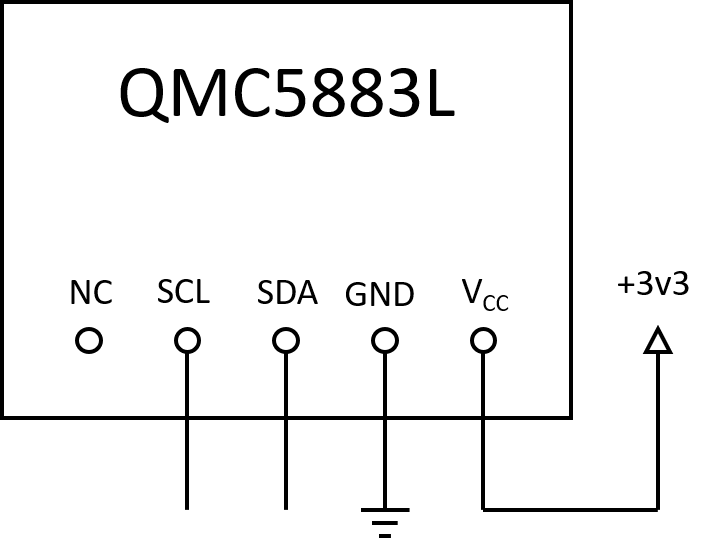
\includegraphics[width=\textwidth]{./img/QMC5883L_Plan.png}
  \caption{Verschaltung des QMC5883L}\label{fig:QMC5883L_Plan}
\end{figure}

Da der Sensor das Magnetfeld misst, muss dieser entfernt von der Windfahne und dem Anemometer platziert werden, da beide mit magnetischen Bauteilen arbeiten. Andernfalls könnte es zu Fehlmessungen kommen. Umgesetzt wurde dies so, dass an der einen Stütze des Solarpanels das Kompassmodul und an der anderen die Windfahne, das Anemometer und das gegenüber magnetischen Beeinflussungen relativ unempfindliche GPS-Modul angebracht wurden. % Verweis auf noch einzufügendes Bild der Montage

%\begin{figure}[H]
% \centering
%  \includegraphics[width=\textwidth]{./img/Montage.png}
%  \caption{Verschaltung des QMC5883L}\label{fig:Montage}
%\end{figure}

\subsection{GPS}

\subsubsection{C-Code}

\subsubsection{Montage}

\subsection{Anemometer}

Viel gut als alte, voll simpel, much wow

\subsubsection{C-Code}

\subsubsection{Montage}

\subsection{Neigungssensor MPU6050}

\subsubsection{C-Code}

\subsubsection{Montage}

\begin{figure}[H]
  \centering
  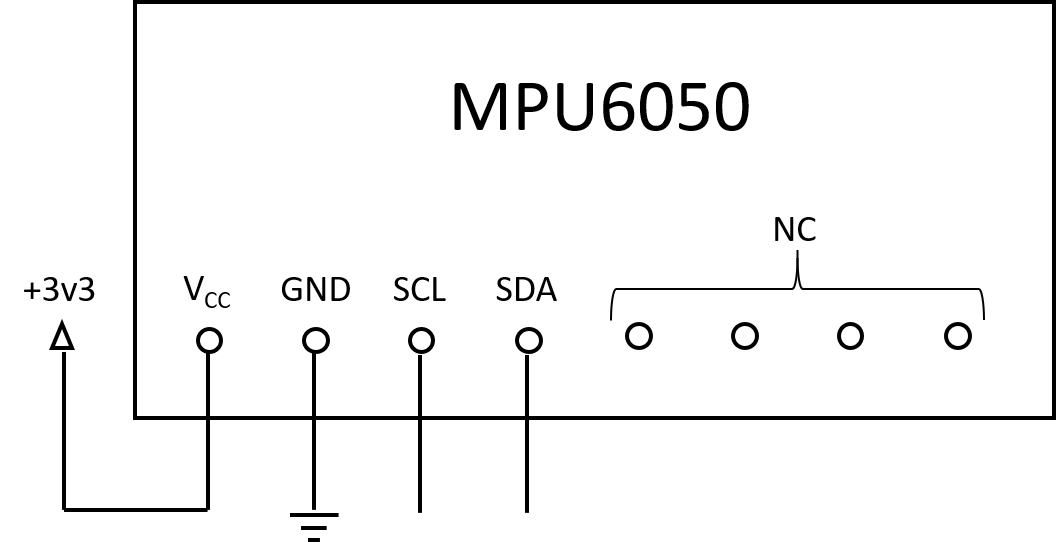
\includegraphics[width=\textwidth]{./img/MPU6050_Plan.png}
  \caption{Verschaltung des MPU6050}\label{fig:MPU6050_Plan}
\end{figure}

\subsection{BME280}

\subsubsection{C-Code}

\subsubsection{Montage}

\begin{figure}[H]
  \centering
  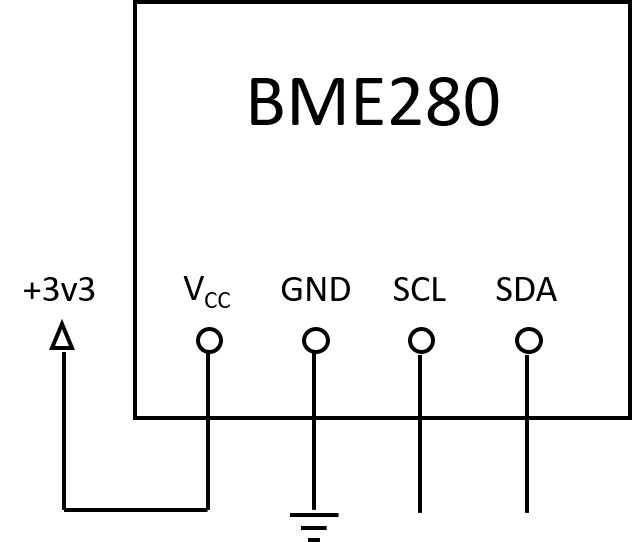
\includegraphics[width=\textwidth]{./img/BME280_Plan.png}
  \caption{Verschaltung des BME280}\label{fig:BME280_Plan}
\end{figure}
